\documentclass[11pt]{article}
\usepackage[T1,T2A]{fontenc}
\usepackage[utf8]{inputenc}
\usepackage[english,russian]{babel}
\usepackage{graphicx}
\usepackage{amsmath}
\graphicspath {{img/}}

\title{\textbf{Лабораторная работа №6\\<<Помехоустойчивое кодирование. Код Хэмминга>>}}
\author{Перепелица А.А., ККСО-01-19}
\date{Москва, 2022 г.}
\addtolength{\topmargin}{-3cm}
\addtolength{\textheight}{3cm}
\begin{document}
\maketitle
\thispagestyle{empty}
\textbf{Цель работы:}  ознакомление с принципами помехоустойчивого кодирования и приобретение практических навыков моделирования работы кодеров и декодеров. 

\section{Задание №1: формирование бита чётности}

\subsection{Формирование бита чётности}
Сформировать бит чётности (бит паритета) для заданного байта передаваемых данных. Исходными данными является последовательность 10111010 (15-й вариант).

Паритетный бит $k$ для n-битного двоичного слова $b_n \ldots b_2 b_1$ вычисляется по формуле:
$$
k=b_n \oplus \ldots \oplus b_2 \oplus b_1
$$

Таким образом, число единиц в последовательности будет всегда чётным. Для нашего примера получим выражение:
$$
k= 1 \oplus 0 \oplus 1\oplus 1\oplus 1\oplus 0\oplus 1\oplus 0 = 1
$$
Тогда $k=1$, кодовая комбинация будет равна: 101110101.

\newpage

\section{Задание №2: Исследование помехоустойчивого кода с формированием бита чётности}

\subsection{Исходные данные для задания}

\begin{table}[h]
    \resizebox{\textwidth}{!}{%
    \begin{tabular}{lllll}
    \hline
    \multicolumn{1}{|c|}{Информационные биты $S_1$, $S_2$, $S_3$, $S_4$} & \multicolumn{1}{c|}{Помехи $S_8$, $S_7$, $S_6$, $S_5$} & \multicolumn{1}{c|}{Помехи $S_8$, $S_7$, $S_6$, $S_5$} & \multicolumn{1}{c|}{Помехи $S_8$, $S_7$, $S_6$, $S_5$} & \multicolumn{1}{c|}{Помехи $S_8$, $S_7$, $S_6$, $S_5$} \\ \hline
    \multicolumn{1}{|c|}{1110} & \multicolumn{1}{c|}{0000} & \multicolumn{1}{c|}{0010} & \multicolumn{1}{c|}{1100} & \multicolumn{1}{c|}{1011} \\ \hline
                           &                       &                       &                       &                       \\
                           &                       &                       &                       &                      
    \end{tabular}%
    }
    \end{table}
\begin{center}
    Таблица 1 - Исходные данные для задания №2
\end{center}

\subsection{ Перечень элементов, использованных в схемах, с их краткими характеристиками}
\begin{itemize}
    \item[-] XOR5 
    \item[-] XOR4
    \item[-] XOR2 - 4 шт.
    \item[-] Цифровой источник питания
    \item[-] Ключ - 8 шт.
    \item[-] Индикатор - 2 шт.
\end{itemize}
\subsection{Схема для моделирования процесса передачи информации по каналу связи}

\begin{center}
    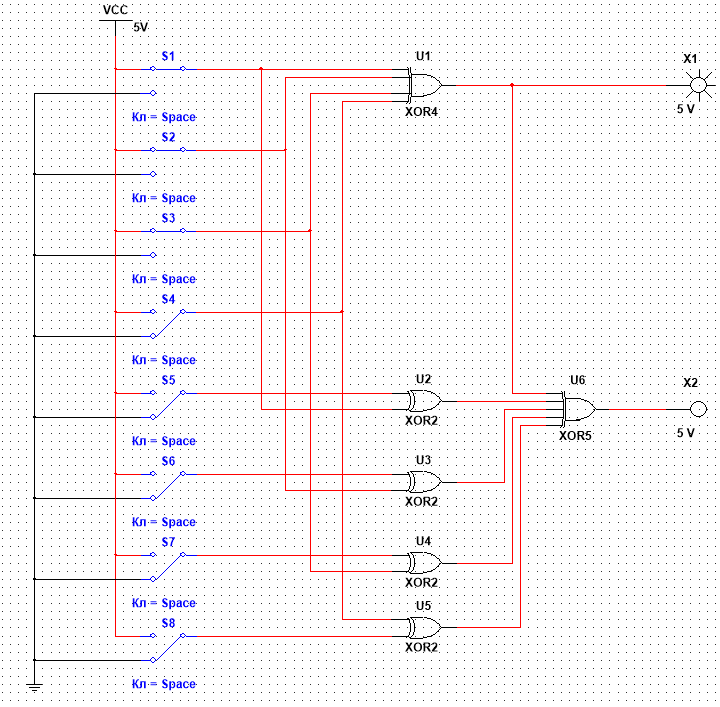
\includegraphics[width=1\linewidth]{img/scheme1.png}
    Рис. 1 - Схема для исследования кода с формированием бита чётности
\end{center}

\subsection{Результаты расчетов}
\begin{center}
    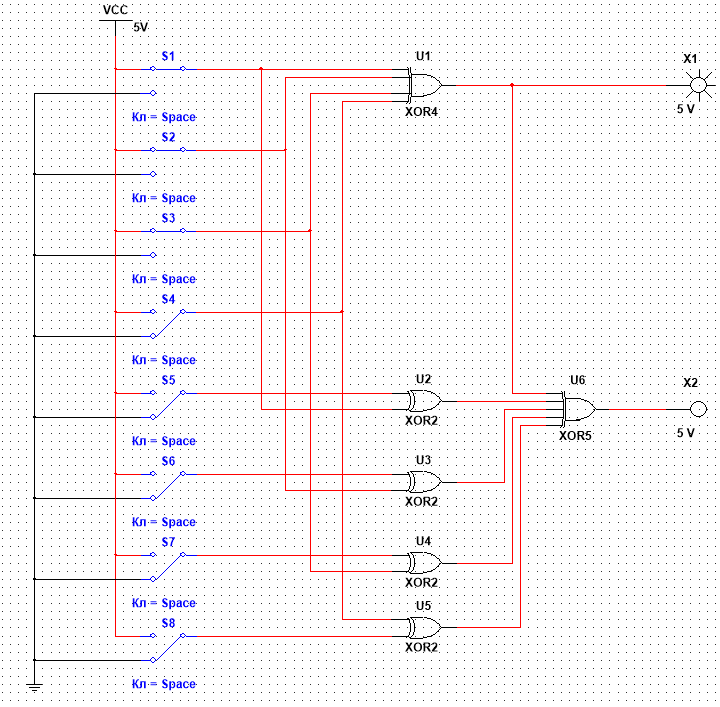
\includegraphics[width=1\linewidth]{img/scheme1.png}
    Рис. 2 - Схема при первой помехе - 0000.
\end{center}

\begin{center}
    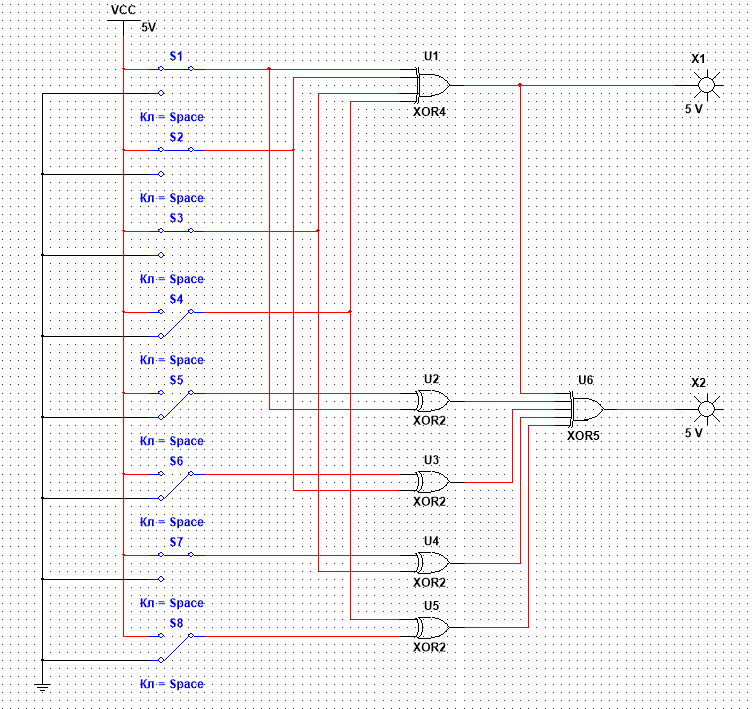
\includegraphics[width=1\linewidth]{img/pomeha2.png}
    Рис. 3 - Схема при второй помехе - 0010.
\end{center}

\begin{center}
    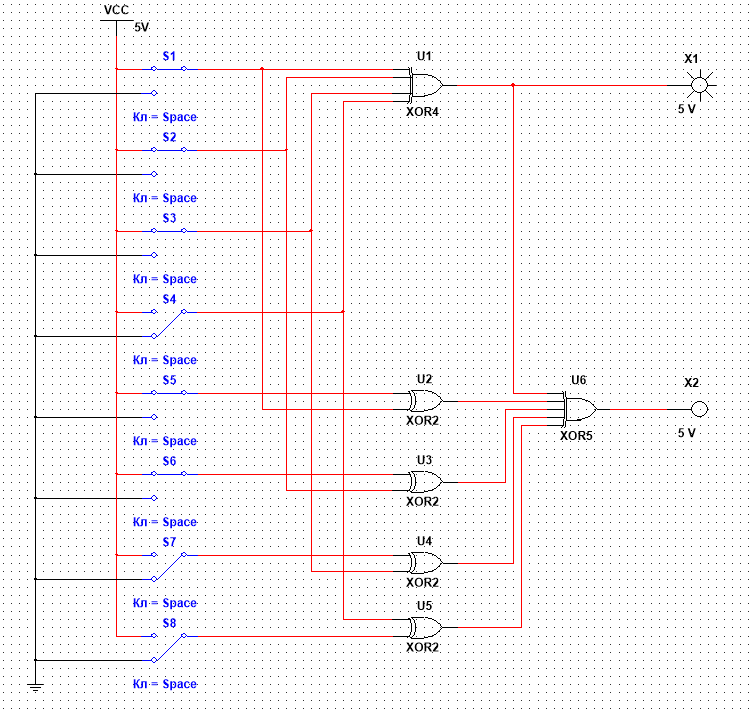
\includegraphics[width=1\linewidth]{img/pomeha3.png}
    Рис. 4 - Схема при третьей помехе - 1100.
\end{center}

\begin{center}
    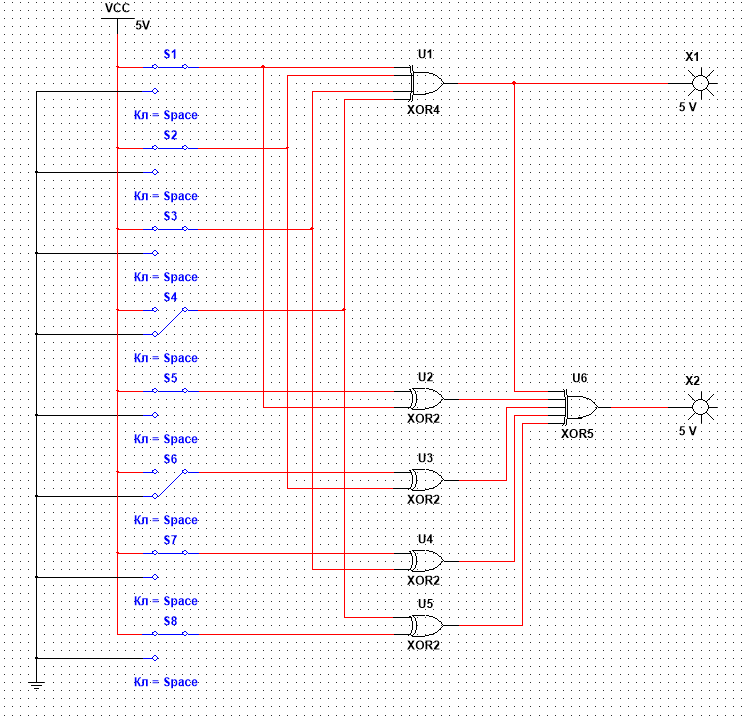
\includegraphics[width=1\linewidth]{img/pomeha4.png}
    Рис. 5 - Схема при четвертой помехе - 1011.
\end{center}

\newpage
\section{Задание №3: Исправление ошибки с помощью кода Хэмминга}
Расчётным путём, точнее вручную, определим, в каком разряде кода Хэмминга произошло искажение. 
\subsection{Исходные данные для задания}
\begin{table}[h]
    \resizebox{\textwidth}{!}{%
    \begin{tabular}{llllllllllll}
    \hline
    \multicolumn{1}{|c|}{$i_8$} & \multicolumn{1}{c|}{$i_7$} & \multicolumn{1}{c|}{$i_6$} & \multicolumn{1}{c|}{$i_5$} & \multicolumn{1}{c|}{$k_4$} & \multicolumn{1}{c|}{$i_4$} & \multicolumn{1}{c|}{$i_3$} & \multicolumn{1}{c|}{$i_2$} & \multicolumn{1}{c|}{$k_3$} & \multicolumn{1}{c|}{$i_1$} & \multicolumn{1}{c|}{$k_2$} & \multicolumn{1}{c|}{$k_1$} \\ \hline
    \multicolumn{1}{|c|}{1} & \multicolumn{1}{c|}{0} & \multicolumn{1}{c|}{1} & \multicolumn{1}{c|}{0} & \multicolumn{1}{c|}{0} & \multicolumn{1}{c|}{1} & \multicolumn{1}{c|}{1} & \multicolumn{1}{c|}{0} & \multicolumn{1}{c|}{0} & \multicolumn{1}{c|}{1} & \multicolumn{1}{c|}{0} & \multicolumn{1}{c|}{0} \\ \hline
                           &                       &                       &                       &                       &                       &                       &                       &                       &                       &                       &                       \\
                           &                       &                       &                       &                       &                       &                       &                       &                       &                       &                       &                      
    \end{tabular}%
    }
    \end{table}
\begin{center}
        Таблица 2 - Исходные данные для задания №3.
\end{center}

\subsection{Процесс вычисления искажённого бита}
Найдём значения k-х битов на приеме:

$k'_1 = i_3 \oplus i_5 \oplus i_7 \oplus i_9 \oplus i_{11} = 1 \oplus$ \\

$k'_2 = i_3 \oplus i_6 \oplus i_7 \oplus i_{10} \oplus i_{11} = 1 \oplus$ \\

$k'_3 = i_5 \oplus i_6 \oplus i_7 \oplus i_{12} = 1 \oplus$ \\

$k'_4 = i_9 \oplus i_{10} \oplus i_{11} \oplus i_{12}= 1 \oplus$

k-е биты на передающей принимающей стороне отличаются, что
свидетельствует о наличие ошибки.

\newpage
\section{Задание №4: Моделирование работы кода Хэмминга}
\subsection{Исходные данные для задания}
Исходные данные приведены в таблице 2.
\subsection{Перечень элементов, использованных в схемах, с их краткими характеристиками.}
\begin{itemize}
    \item [-] XOR5 - 4 шт.
    \item [-] XOR4 - 4 шт.
    \item [-] XOR2 - 16 шт.
    \item [-] Цифровой источник питания
    \item [-] Генератор слов
    \item [-] Ключ - 8 шт.
    \item [-] Индикатор - 12 шт.
\end{itemize}
\subsection{Схема для исследования работы кода Хэмминга}
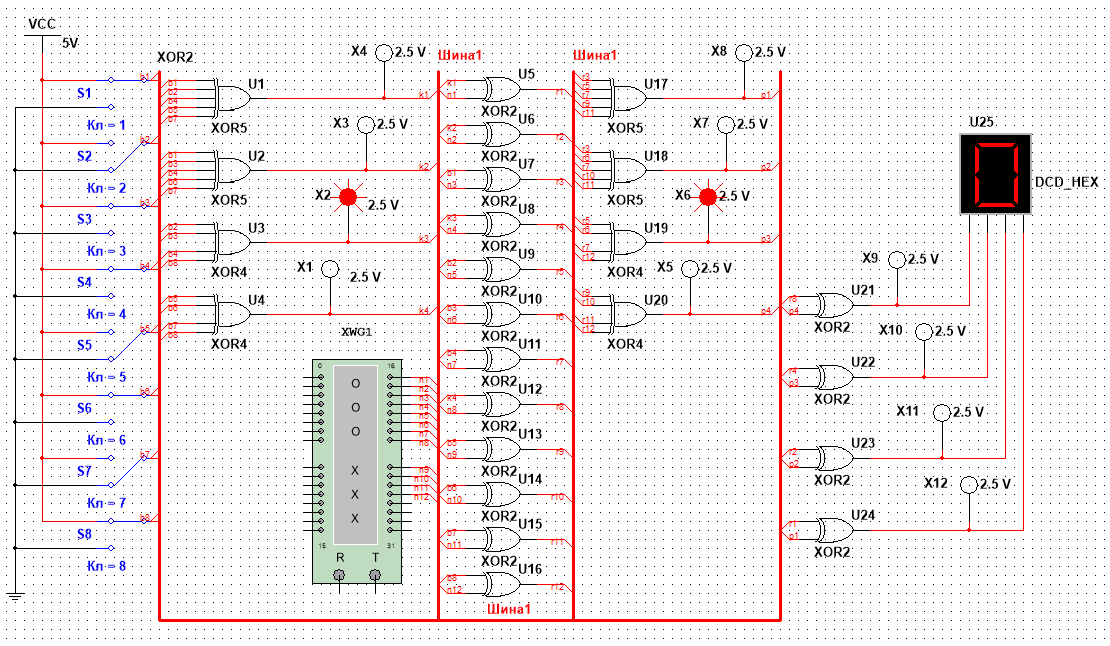
\includegraphics[width=1\linewidth]{img/scheme2.png}
\begin{center}
        Рис 6 - Схема моделирования работы кода Хэмминга в системе передачи информации.
\end{center}

\subsection{Результаты расчётов}
Ниже представлена таблица помех и показаний схемы моделирования работы кода Хэмминга:

\begin{table}[h]
    \resizebox{\textwidth}{!}{
    \begin{tabular}{|l|l|l|}
    \hline
    \multicolumn{1}{|c|}{В каком бите искажение}     & \multicolumn{1}{c|}{Значения контрольных битов на приёмнике} & \multicolumn{1}{c|}{Синдром} \\ \hline
    \multicolumn{1}{|c|}{$k_1$} & \multicolumn{1}{c|}{} & \multicolumn{1}{c|}{} \\ \hline
    \multicolumn{1}{|c|}{$k_2$}                       &\multicolumn{1}{|c|}{}                       &\multicolumn{1}{|c|}{}                       \\ \hline
    \multicolumn{1}{|c|}{$i_1$}                       &\multicolumn{1}{|c|}{}                       &\multicolumn{1}{|c|}{}                       \\ \hline
    \multicolumn{1}{|c|}{$k_3$}                       &\multicolumn{1}{|c|}{}                       &\multicolumn{1}{|c|}{}                       \\ \hline
    \multicolumn{1}{|c|}{$i_2$}                       &\multicolumn{1}{|c|}{}                       &\multicolumn{1}{|c|}{}                       \\ \hline
    \multicolumn{1}{|c|}{$i_3$}                       &\multicolumn{1}{|c|}{}                       &\multicolumn{1}{|c|}{}                       \\ \hline
    \multicolumn{1}{|c|}{$k_4$}                       &\multicolumn{1}{|c|}{}                       &\multicolumn{1}{|c|}{}                       \\ \hline
    \multicolumn{1}{|c|}{$i_4$}                       &\multicolumn{1}{|c|}{}                       &\multicolumn{1}{|c|}{}                       \\ \hline
    \multicolumn{1}{|c|}{$i_5$}                       &\multicolumn{1}{|c|}{}                       &\multicolumn{1}{|c|}{}                       \\ \hline
    \multicolumn{1}{|c|}{$i_6$}                       &\multicolumn{1}{|c|}{}                       &\multicolumn{1}{|c|}{}                       \\ \hline
    \multicolumn{1}{|c|}{$i_7$}                       &\multicolumn{1}{|c|}{}                       &\multicolumn{1}{|c|}{}                       \\ \hline
    \multicolumn{1}{|c|}{$i_8$}                       &\multicolumn{1}{|c|}{}                       &\multicolumn{1}{|c|}{}                       \\ \hline
    \end{tabular}
    }
    \end{table} \\


Проведём анализ результатов кода с проверкой на чётность:

\begin{table}[h]
    \resizebox{\textwidth}{!}{%
    \begin{tabular}{|l|l|l|}
    \hline
    \multicolumn{1}{|c|}{В каком бите искажение}     & \multicolumn{1}{c|}{Бит чётности на кодере} & \multicolumn{1}{c|}{Бит чётности на приёме} \\ \hline
    \multicolumn{1}{|c|}{$k_1$} & \multicolumn{1}{c|}{} & \multicolumn{1}{c|}{} \\ \hline
    \multicolumn{1}{|c|}{$k_2$}                       &\multicolumn{1}{|c|}{}                       &\multicolumn{1}{|c|}{}                       \\ \hline
    \multicolumn{1}{|c|}{$i_1$}                       &\multicolumn{1}{|c|}{}                       &\multicolumn{1}{|c|}{}                       \\ \hline
    \multicolumn{1}{|c|}{$k_3$}                       &\multicolumn{1}{|c|}{}                       &\multicolumn{1}{|c|}{}                       \\ \hline
    \multicolumn{1}{|c|}{$i_2$}                       &\multicolumn{1}{|c|}{}                       &\multicolumn{1}{|c|}{}                       \\ \hline
    \multicolumn{1}{|c|}{$i_3$}                       &\multicolumn{1}{|c|}{}                       &\multicolumn{1}{|c|}{}                       \\ \hline
    \multicolumn{1}{|c|}{$k_4$}                       &\multicolumn{1}{|c|}{}                       &\multicolumn{1}{|c|}{}                       \\ \hline
    \multicolumn{1}{|c|}{$i_4$}                       &\multicolumn{1}{|c|}{}                       &\multicolumn{1}{|c|}{}                       \\ \hline
    \multicolumn{1}{|c|}{$i_5$}                       &\multicolumn{1}{|c|}{}                       &\multicolumn{1}{|c|}{}                       \\ \hline
    \multicolumn{1}{|c|}{$i_6$}                       &\multicolumn{1}{|c|}{}                       &\multicolumn{1}{|c|}{}                       \\ \hline
    \multicolumn{1}{|c|}{$i_7$}                       &\multicolumn{1}{|c|}{}                       &\multicolumn{1}{|c|}{}                       \\ \hline
    \multicolumn{1}{|c|}{$i_8$}                       &\multicolumn{1}{|c|}{}                       &\multicolumn{1}{|c|}{}                       \\ \hline
    \end{tabular}%
    }
    \end{table} \\

    
Анализ результата кода с проверкой на чётность показывает наличие ошибки, однако не указывает на её местоположение.


\textbf{Вывод:} В ходе работы были изучены теоретические аспекты помехоустойчивого кодирования, а также приобретены практические навыки моделирования работы кода Хэмминга.

\end{document}